% Created 2023-11-08 mié 00:48
% Intended LaTeX compiler: pdflatex
\documentclass[11pt]{article}
\usepackage[utf8]{inputenc}
\usepackage[T1]{fontenc}
\usepackage{graphicx}
\usepackage{longtable}
\usepackage{wrapfig}
\usepackage{rotating}
\usepackage[normalem]{ulem}
\usepackage{amsmath}
\usepackage{amssymb}
\usepackage{capt-of}
\usepackage{hyperref}
\usepackage{../../modern}
\bibliography{./fuentes.bib}
\raggedbottom
\setcounter{secnumdepth}{2}
\author{Luis Eduardo Galindo Amaya (1274895)}
\date{martes, 07 noviembre 2023}
\title{Práctica No. 4 Laboratorio}
\hypersetup{
 pdfauthor={Luis Eduardo Galindo Amaya (1274895)},
 pdftitle={Práctica No. 4 Laboratorio},
 pdfkeywords={},
 pdfsubject={},
 pdfcreator={Emacs 28.1 (Org mode 9.5.2)}, 
 pdflang={Spanish}}
\begin{document}

\modentitlepage{../../images/escudo-uabc-2022-1-tinta-pos.png}
\datasection{Individual}
\tableofcontents
\pagebreak

\section{Introducción}
\label{sec:orgf522a28}
A lo largo de esta practica utizaré la Lógica de primer orden para
implementar la red semántica de la practica pasada. Acorde a wikipedia
la logica de primer orden: \\

\ldots{}Es un sistema formal diseñado para estudiar la inferencia en los
lenguajes de primer orden. Los lenguajes de primer orden son, a su
vez, lenguajes formales con cuantificadores que alcanzan solo a
variables de individuo, y con predicados y funciones cuyos argumentos
son solo constantes o variables de individuo\autocite{Wikipedia_2023}.

\section{Red Semantica de conocimiento personal}
\label{sec:orgc5e3a43}
La red semántica de la practica anterior, en esta red podemos
identificar las relaciones entre los diversos conceptos

\begin{figure}[htbp]
\centering
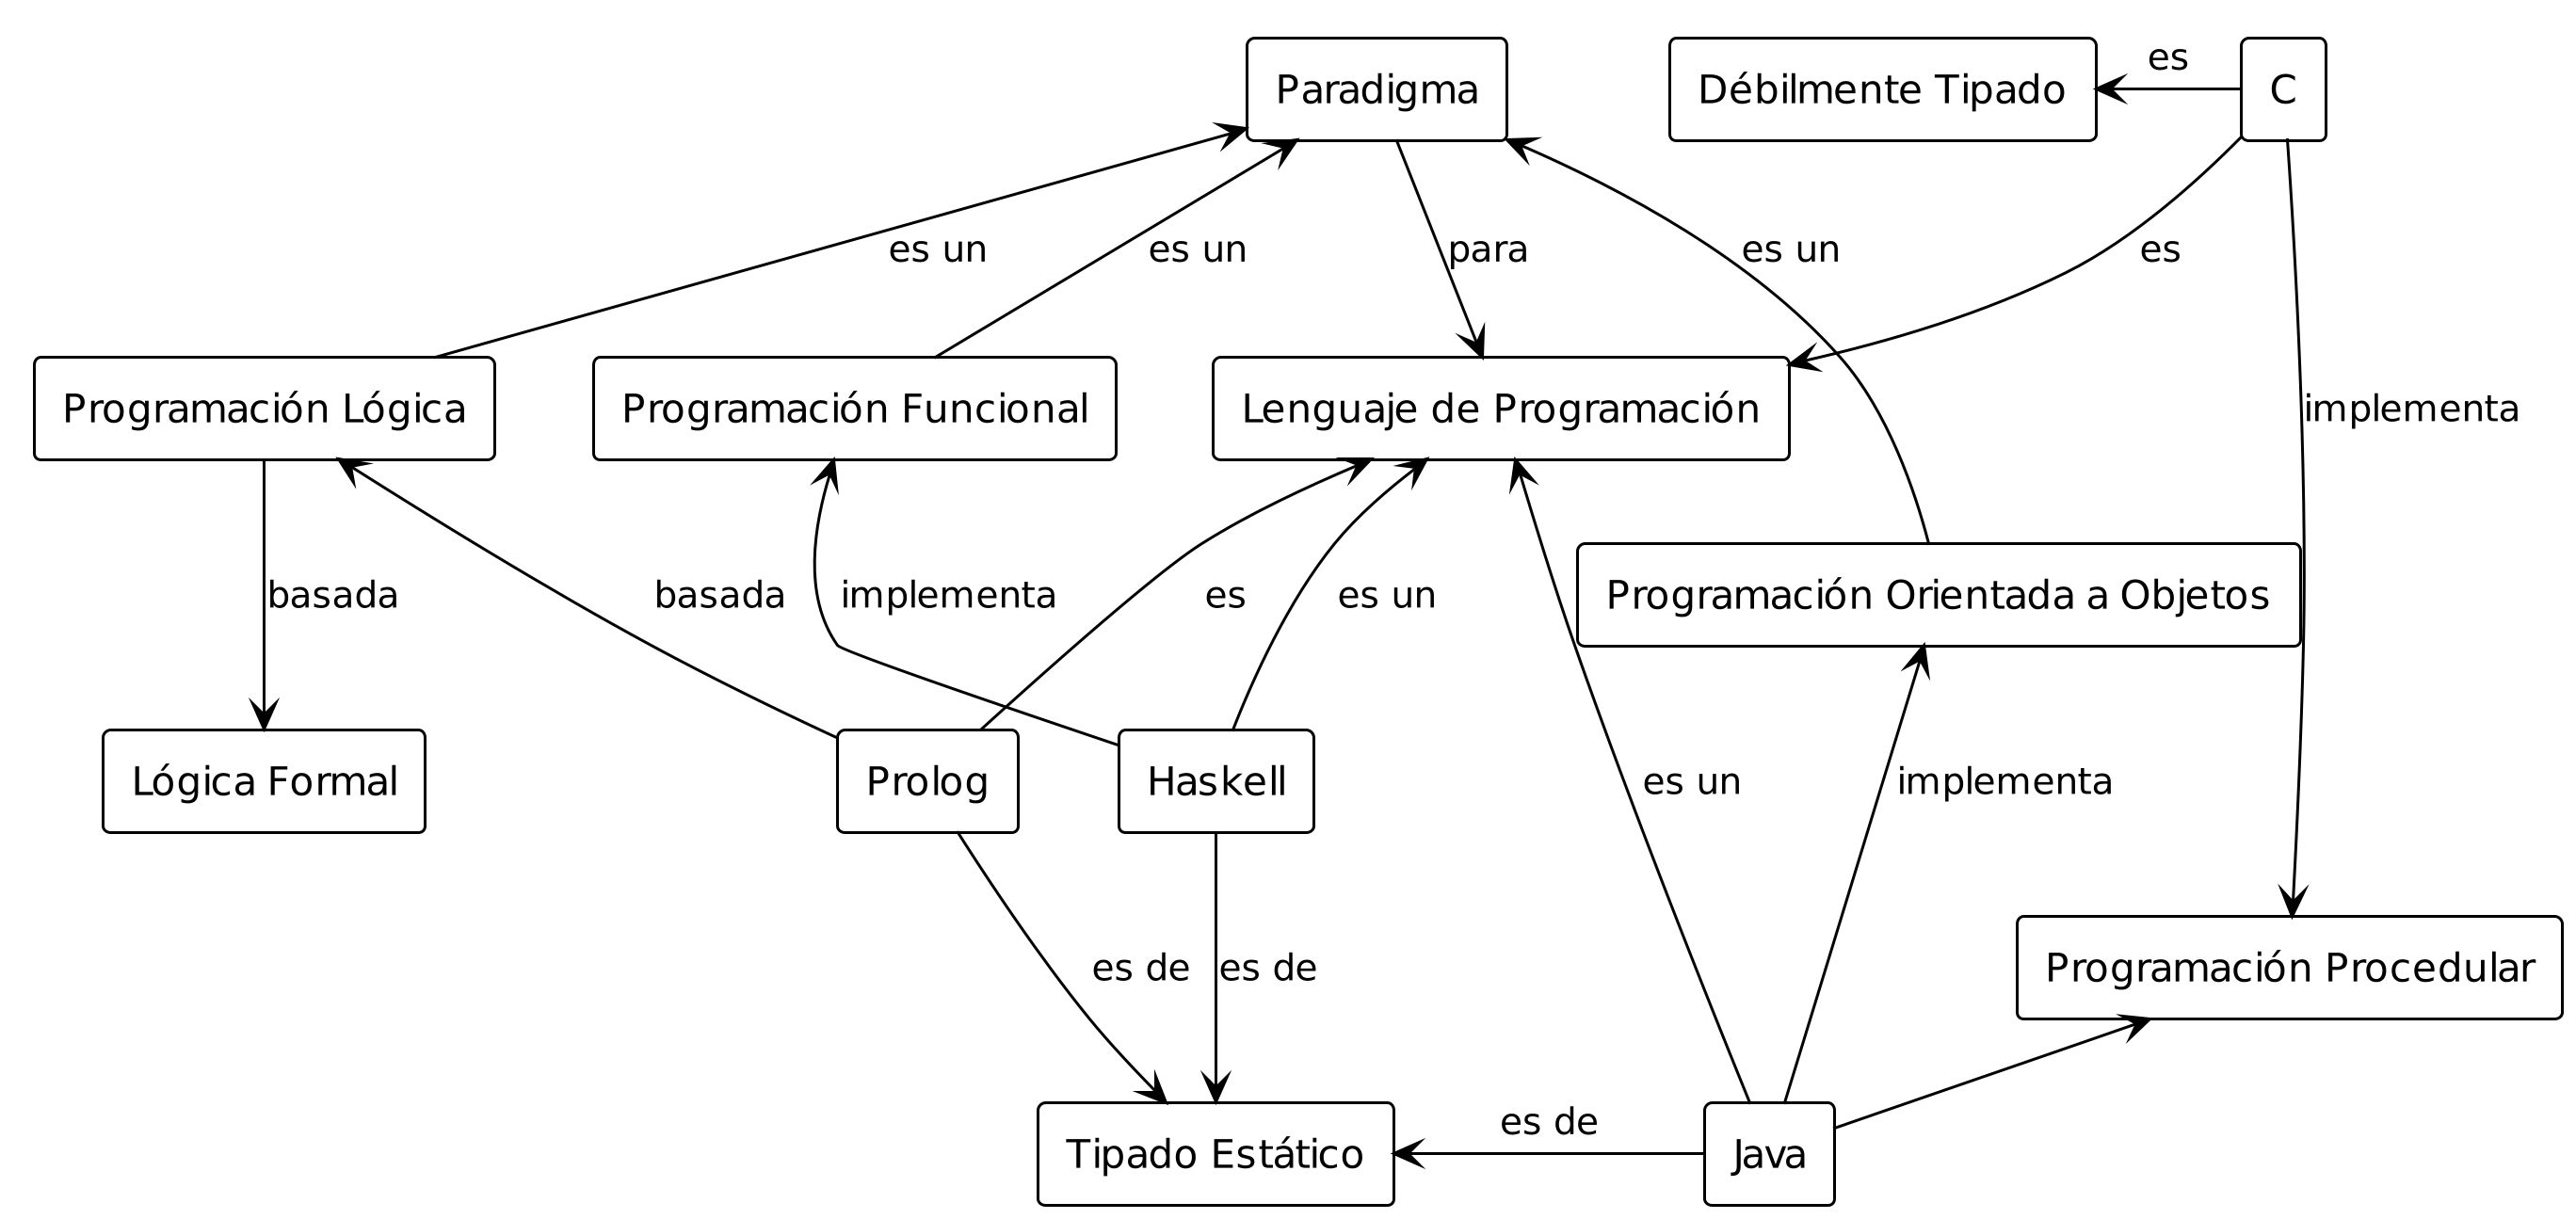
\includegraphics[width=.9\linewidth]{./img/test.png}
\caption{Red semántica de 'Lenguajes y Paradigmas' de la pagina anterior.}
\end{figure}

\section{Formalizar la representación}
\label{sec:org6aa1b95}
\[\begin{align*}
\text{Variables} & & \text{Hechos} \\
P &= \text{Paradigma} & P(PF) \\
L &= \text{Lenguaje de programación} & P(PL) \\
TT &= \text{Tipo de Tipado} & P(PE) \\
B &= \text{Basada} & P(POO) \\
I &= \text{Implementa} & L(PG) \\
TE &= \text{Tipado Estatico} & L(HS) \\
LF &= \text{Lógica formal} & L(J)\\
PF &= \text{Programacion funcional} & L(C) \\
PL &= \text{Programacion logica} & I(J,POO) \\
PE &= \text{Programacion estructurada} & I(J,PE) \\
POO &= \text{Programacion Oriendad a Objetos} & B(PL,LF) \\
PG &= \text{Prolog} & I(PG,PL) \\
HS &= \text{Haskell} & I(C,PE) \\
J &= \text{Java} & TD(C) \\
C &= \text{C} & TE(HS) \\
TD &= \text{Tipado Debil} & TE(PG) \\
& & I(HS,PF) 
\end{align*}\]

\begin{description}
\item[{\(T(E) \land P(PF) \implies HS\)}] Sí es de tipado estatico y de
paradigma funcional entonces el lenguaje es Haskell.

\item[{\(I(L, POO) \land I(L, PE) \implies J\)}] Sí el lenguaje
implementa el paradigma orientado a objetos y el prardigma
estructurado entonces el lenguaje es Java.

\item[{\(I(L, PE) \land TD(L) \implies C\)}] Si el lenguaje implementa
el paradigma procedular y de tipado debil entonces el lenguaje es C.

\item[{\(T(E) \land P(PL) \implies PG\)}] Sí es de tipado estatico y de
paradigma Logico entonces el lenguaje es Prolog.
\end{description}

\section{Conclusión}
\label{sec:orgbdd7c05}
En esta práctica, hemos utilizado la lógica de primer orden para
formalizar la representación de una red semántica de conocimiento
personal. A través de esta formalización, hemos establecido una
serie de reglas lógicas que nos permiten inferir información sobre los
lenguajes de programación en función de sus características y
relaciones con los paradigmas de programación. 

\section{Referencias}
\label{sec:orgb880590}
\printbibliography[heading=none]
\end{document}